% !TeX TS-program = xelatex
\documentclass[12pt]{article}
\usepackage{listings}
\usepackage{float}
\usepackage{xcolor}
\usepackage{graphicx}
\usepackage{booktabs}
\usepackage{marginnote}
\usepackage{caption}
\definecolor{codegreen}{rgb}{0,0.6,0}
\definecolor{codegray}{rgb}{0.5,0.5,0.5}
\definecolor{codepurple}{rgb}{0.58,0,0.82}
\definecolor{backcolour}{rgb}{0.95,0.95,0.92}
\lstdefinestyle{mystyle}{
	backgroundcolor=\color{backcolour},   commentstyle=\color{codegreen},
	keywordstyle=\color{magenta},
	numberstyle=\tiny\color{codegray},
	stringstyle=\color{codepurple},
	basicstyle=\ttfamily\footnotesize,
	breakatwhitespace=false,
	breaklines=true,
	captionpos=b,
	keepspaces=true,
	numbers=left,
	numbersep=5pt,
	showspaces=false,
	showstringspaces=false,
	showtabs=false,
	tabsize=2
}
%"mystyle" code listing set
\lstset{style=mystyle}
%\lstset{basicstyle=\ttfamily\footnotesize,breaklines=true}

\usepackage[breaklinks]{hyperref}
% Setup de hiperenlaces
\hypersetup{
	colorlinks=true,
	linkcolor=blue,
	filecolor=magenta,
	urlcolor=cyan,
	pdftitle={Apuntes de Consolas y Videojuegos},
	pdfpagemode=FullScreen,
	citecolor = green
}

\usepackage{url}

\usepackage{fontspec}
\setmainfont{AT-NameSansText}[
	Path=./NameSansStatic/,
	Extension = .otf,
	UprightFont=*-Regular,
	BoldFont=*-Bold,
	ItalicFont=*-RegularItalic,
	BoldItalicFont=*-BoldItalic,
	Numbers = OldStyle
]

\setmonofont{ATNameMono}[
	Path=./NameMonoStatic/,
	Extension = .otf,
	UprightFont=*-Regular,
	BoldFont=*-Bold,
	ItalicFont=*-RegularItalic,
	BoldItalicFont=*-BoldItalic
]

\usepackage[backend=biber]{biblatex}
\addbibresource{referencias.bib}
\usepackage{notoccite}
\renewcommand{\figurename}{\textbf{Figura.}}
\renewcommand{\tablename}{\textbf{Tabla.}}

\begin{document}
\nocite{namesans_about}
\nocite{namesans}
\nocite{namemono}


	\begin{titlepage}
		\begin{center}
			{\Huge \textbf{Entregable de Teoría 10}}

			\vspace{2cm}

			{\Large \textit{Jesús Jiménez Montero}}

			\vspace{2cm}
		\end{center}
	\end{titlepage}

	% ÍNDICE
	%\renewcommand{\tableofcontents}{Indice general}
	\newpage
	\renewcommand{\contentsname}{Tabla de contenidos}
	\setcounter{secnumdepth}{5}
	\tableofcontents
	\setcounter{tocdepth}{4}
	\newpage

\section{Introducción a la jerarquía de memoria} \cite{patterson-2011}
	El sistema de la memoria de un ordenador se ordena mediante una jerarquía establecida, la cual hace pensar al usuario de que dispone una memoria muy grande a la cual se puede acceder muy rápidamente.\\
	Esta jerarquía establece que los programas acceden a una parte del espacio de direcciones en un instante determinado, lo que lleva a la creación del principio de localidad:
	\begin{itemize}
		\item \textbf{Localidad temporal (en el tiempo)}: Si se accede a una dirección de memoria, existe la posibilidad de ser usada de nuevo en un plazo corto de tiempo.
		\item \textbf{Localidad espacial (en el espacio)}: Si se accede a una dirección de memoria, las direcciones más cercanas a la accedida, son más probables de ser utilizadas de nuevo.
	\end{itemize}

	Para construir esta jerarquía se hace tal manera:
	% Please add the following required packages to your document preamble:
	% \usepackage{booktabs}
	% \usepackage{graphicx}
	\begin{table}[H]
		\centering
		\caption{Estructura básica de la jerarquía de memoria}
		\label{tab:jerarq_mem}
		\resizebox{\textwidth}{!}{%
		\begin{tabular}{@{}lllll@{}}
		\toprule
		Velocidad  & CPU     & Capacidad & Coste    & Tecnología      \\ \midrule
		Más rapida & Memoria & Menor     & Más alta & SRAM            \\
				& Memoria &           &          & DRAM            \\
		Más baja   & Memoria & Mayor     & Más baja & Disco magnético \\ \bottomrule
		\end{tabular}%
		}
	\end{table}

	Cuando el procesador busca datos, se accede según el orden establecido en la jerarquía. Si al buscar estos datos en una memoria de nivel superior (más rápida) y se encuentra en esta, se considera un acierto; y si no se encuentran, se considera un fallo.\\

	El tiempo de acierto es el tiempo necesario para acceder a la memoria de nivel superior, y la penalización por fallo es el tiempo necesario para acceder a la memoria de nivel inferior y traer los datos a la memoria de nivel superior.

\section{Memoria Caché} \cite{patterson-2011}
	La caché es una memoria especial situada entre la CPU y la memoria principal que almacena los datos e instrucciones que se usan con más frecuencia. El uso principal de la caché es reducir el tiempo medio que toma en acceder a los datos de la memoria principal. \cite{geeksforgeeks-2023} \\

	\subsection{Caché de Correspondencia Directa}
		La forma más sencilla de caché, se denomina correspondencia directa, la cual asigna una posición de la caché basándose en la dirección de memoria.\footnote{\textit{Cache de correspondencia directa: organización de cache en la que cada posición de la memoria principal se corresponde con una única posición de la cache.}}

		Para poder alojar el contenido de varias posiciones diferentes de la memoria principal, se usan las etiquetas, las cuales llevan la información de la direccion necesaria para identificar si una palabra de la caché se corresponde con una palabra de la memoria principal.

		\begin{figure}[H]
			\centering
			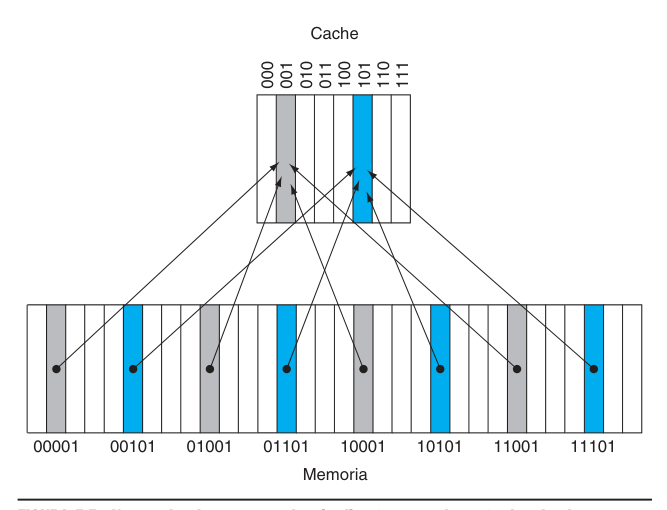
\includegraphics[width=0.65\linewidth]{Imagenes/cache_correspodencia_directa}
			\caption{Ejemplo de funcionamiento de caché de correspondencia básica. Los ultimos 3 bits significativos hacen referencia a en que ranura de la cache se encuentra mapeada la RAM.\\
			\textit{Figura cortesía de \cite{patterson-2011}}}
			\label{fig:cachecorrespodenciadirecta}
		\end{figure}

		También se necesita una forma de comprobar si la información de una cache es valida o no, un programa puede solicitar una información que no tiene sentido para este y las etiquetas no sirve o las entradas de la cache pueden estar vacías. Se usa el bit de validez para estoo, el cual indica si la información de la cache es valida o no.\\

		\begin{figure}[H]
			\centering
			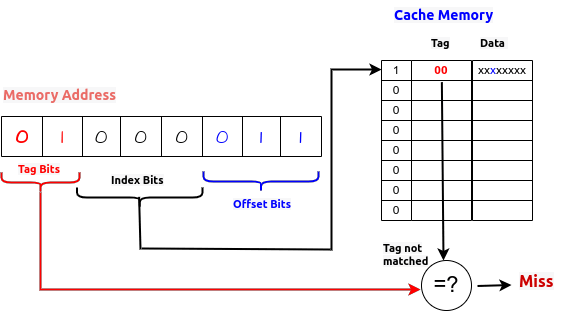
\includegraphics[width=0.75\linewidth]{Imagenes/ejemplo_corresp_directa}
			\caption{Ejemplo del funcionamiento de una memoria de 8-bit y cache de 8 ranuras.\\
			Figura cortesía de \cite{kumar-2023}}
			\label{fig:ejemplocorrespdirecta}
		\end{figure}



\newpage

\printbibliography[title={Bibliografía y agradecimientos}]
\end{document}